% !TeX program = pdflatex
% !TeX root = GAE.tex

\documentclass[../FeynCalcManual.tex]{subfiles}
\begin{document}
\hypertarget{gae}{
\section{GAE}\label{gae}\index{GAE}}

\texttt{GAE[\allowbreak{}mu]} can be used as input for a
\texttt{D-4}-dimensional \(\gamma^{\mu }\)and is transformed into
\texttt{DiracGamma[\allowbreak{}LorentzIndex[\allowbreak{}mu,\ \allowbreak{}D-4],\ \allowbreak{}D-4]}
by \texttt{FeynCalcInternal} (\texttt{FCI}).

\texttt{GAE[\allowbreak{}mu,\ \allowbreak{}nu ,\ \allowbreak{}...]} is a
short form for \texttt{GAE[\allowbreak{}mu].GAE[\allowbreak{}nu] ...}.

\subsection{See also}

\hyperlink{toc}{Overview}, \hyperlink{diracgamma}{DiracGamma},
\hyperlink{ga}{GA}, \hyperlink{gs}{GS}, \hyperlink{gad}{GAD}.

\subsection{Examples}

\begin{Shaded}
\begin{Highlighting}[]
\NormalTok{GAE}\OperatorTok{[}\SpecialCharTok{\textbackslash{}}\OperatorTok{[}\NormalTok{Mu}\OperatorTok{]]}
\end{Highlighting}
\end{Shaded}

\begin{dmath*}\breakingcomma
\hat{\gamma }^{\mu }
\end{dmath*}

\begin{Shaded}
\begin{Highlighting}[]
\NormalTok{GAE}\OperatorTok{[}\SpecialCharTok{\textbackslash{}}\OperatorTok{[}\NormalTok{Mu}\OperatorTok{],} \SpecialCharTok{\textbackslash{}}\OperatorTok{[}\NormalTok{Nu}\OperatorTok{]]} \SpecialCharTok{{-}}\NormalTok{ GAE}\OperatorTok{[}\SpecialCharTok{\textbackslash{}}\OperatorTok{[}\NormalTok{Nu}\OperatorTok{],} \SpecialCharTok{\textbackslash{}}\OperatorTok{[}\NormalTok{Mu}\OperatorTok{]]}
\end{Highlighting}
\end{Shaded}

\begin{dmath*}\breakingcomma
\hat{\gamma }^{\mu }.\hat{\gamma }^{\nu }-\hat{\gamma }^{\nu }.\hat{\gamma }^{\mu }
\end{dmath*}

\begin{Shaded}
\begin{Highlighting}[]
\FunctionTok{StandardForm}\OperatorTok{[}\NormalTok{FCI}\OperatorTok{[}\NormalTok{GAE}\OperatorTok{[}\SpecialCharTok{\textbackslash{}}\OperatorTok{[}\NormalTok{Mu}\OperatorTok{]]]]}

\CommentTok{(*DiracGamma[LorentzIndex[\textbackslash{}[Mu], {-}4 + D], {-}4 + D]*)}
\end{Highlighting}
\end{Shaded}

\begin{Shaded}
\begin{Highlighting}[]
\NormalTok{GAE}\OperatorTok{[}\SpecialCharTok{\textbackslash{}}\OperatorTok{[}\NormalTok{Mu}\OperatorTok{],} \SpecialCharTok{\textbackslash{}}\OperatorTok{[}\NormalTok{Nu}\OperatorTok{],} \SpecialCharTok{\textbackslash{}}\OperatorTok{[}\NormalTok{Rho}\OperatorTok{],} \SpecialCharTok{\textbackslash{}}\OperatorTok{[}\NormalTok{Sigma}\OperatorTok{]]}
\end{Highlighting}
\end{Shaded}

\begin{dmath*}\breakingcomma
\hat{\gamma }^{\mu }.\hat{\gamma }^{\nu }.\hat{\gamma }^{\rho }.\hat{\gamma }^{\sigma }
\end{dmath*}

\begin{Shaded}
\begin{Highlighting}[]
\FunctionTok{StandardForm}\OperatorTok{[}\NormalTok{GAE}\OperatorTok{[}\SpecialCharTok{\textbackslash{}}\OperatorTok{[}\NormalTok{Mu}\OperatorTok{],} \SpecialCharTok{\textbackslash{}}\OperatorTok{[}\NormalTok{Nu}\OperatorTok{],} \SpecialCharTok{\textbackslash{}}\OperatorTok{[}\NormalTok{Rho}\OperatorTok{],} \SpecialCharTok{\textbackslash{}}\OperatorTok{[}\NormalTok{Sigma}\OperatorTok{]]]}

\CommentTok{(*GAE[\textbackslash{}[Mu]] . GAE[\textbackslash{}[Nu]] . GAE[\textbackslash{}[Rho]] . GAE[\textbackslash{}[Sigma]]*)}
\end{Highlighting}
\end{Shaded}

\begin{Shaded}
\begin{Highlighting}[]
\NormalTok{GAE}\OperatorTok{[}\SpecialCharTok{\textbackslash{}}\OperatorTok{[}\NormalTok{Alpha}\OperatorTok{]]}\NormalTok{ FVD}\OperatorTok{[}\FunctionTok{p}\OperatorTok{,} \SpecialCharTok{\textbackslash{}}\OperatorTok{[}\NormalTok{Alpha}\OperatorTok{]]} \SpecialCharTok{//}\NormalTok{ Contract}
\end{Highlighting}
\end{Shaded}

\begin{dmath*}\breakingcomma
\hat{\gamma }\cdot \hat{p}
\end{dmath*}

\begin{Shaded}
\begin{Highlighting}[]
\NormalTok{GAE}\OperatorTok{[}\SpecialCharTok{\textbackslash{}}\OperatorTok{[}\NormalTok{Alpha}\OperatorTok{]]}\NormalTok{ FV}\OperatorTok{[}\FunctionTok{p}\OperatorTok{,} \SpecialCharTok{\textbackslash{}}\OperatorTok{[}\NormalTok{Alpha}\OperatorTok{]]} \SpecialCharTok{//}\NormalTok{ Contract}
\end{Highlighting}
\end{Shaded}

\begin{dmath*}\breakingcomma
0
\end{dmath*}

In order to use Dirac algebra with \(D-4\)-dimensional objects you need
to activate the t'Hooft-Veltman-Breitenlohner-Maison scheme first

\begin{Shaded}
\begin{Highlighting}[]
\NormalTok{FCSetDiracGammaScheme}\OperatorTok{[}\StringTok{"NDR"}\OperatorTok{]} 
 
\NormalTok{DiracSimplify}\OperatorTok{[}\NormalTok{GAE}\OperatorTok{[}\SpecialCharTok{\textbackslash{}}\OperatorTok{[}\NormalTok{Mu}\OperatorTok{]]}\NormalTok{ . GAD}\OperatorTok{[}\SpecialCharTok{\textbackslash{}}\OperatorTok{[}\NormalTok{Mu}\OperatorTok{]]]}
\end{Highlighting}
\end{Shaded}

\begin{dmath*}\breakingcomma
\text{NDR}
\end{dmath*}

\FloatBarrier
\begin{figure}[!ht]
\centering
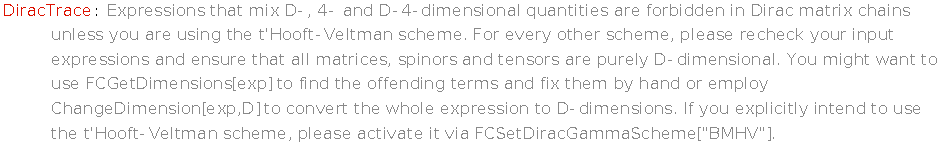
\includegraphics[width=0.6\linewidth]{img/1mv5oz2r1f8id.pdf}
\end{figure}
\FloatBarrier

\begin{dmath*}\breakingcomma
\text{\$Aborted}
\end{dmath*}

\begin{Shaded}
\begin{Highlighting}[]
\NormalTok{FCSetDiracGammaScheme}\OperatorTok{[}\StringTok{"BMHV"}\OperatorTok{]} 
 
\NormalTok{DiracSimplify}\OperatorTok{[}\NormalTok{GAE}\OperatorTok{[}\SpecialCharTok{\textbackslash{}}\OperatorTok{[}\NormalTok{Mu}\OperatorTok{]]}\NormalTok{ . GAD}\OperatorTok{[}\SpecialCharTok{\textbackslash{}}\OperatorTok{[}\NormalTok{Mu}\OperatorTok{]]]}
\end{Highlighting}
\end{Shaded}

\begin{dmath*}\breakingcomma
\text{BMHV}
\end{dmath*}

\begin{dmath*}\breakingcomma
D-4
\end{dmath*}

\begin{Shaded}
\begin{Highlighting}[]
\NormalTok{FCSetDiracGammaScheme}\OperatorTok{[}\StringTok{"NDR"}\OperatorTok{]}
\end{Highlighting}
\end{Shaded}

\begin{dmath*}\breakingcomma
\text{NDR}
\end{dmath*}
\end{document}
